\section{SYSTEM DESCRIPTION}

\subsection{Selecting a Corpus}
The dataset in the task was unavailable. So we emailed on of the organizers and they provided an annotated dataset of similar task\footnote{\url{https://competitions.codalab.org/competitions/23705?secret_key=aeda0cb9-a3da-4e4f-9d6a-d639355b455e}}. This dataset is highly imbalanced. To make it slightly balanced, we collected another dataset used by Alvaro et al.~\cite{alvaro2017twimed}. Both of the dataset were already annotated. We combined the two dataset and generate three datasets for our test purpose. The positive class distribution in these datasets is shown in table~\ref{table:2}. We also come up with a pre-compiled list of 89 medication and dietary names and their variations based on the provided dataset.

\begin{table}[h!]
	\centering
	\begin{tabular}{||c c c||} 
		\hline
		Total Entry & Positive-class & Positive-class percentage \\ [0.5ex] 
		\hline\hline
		52259 & 200 & 0.38 \% \\ 
		52559 & 500 & 0.95 \% \\
		53059 & 1000 & 1.88 \% \\
		\hline
	\end{tabular}
	\caption{Dataset Distribution}
	\label{table:2}
\end{table}

\subsection{Pre-processing}
Tweets are often informal. So preprocessing the data is essential. To do preprocessing, we setup some rules: 
\begin{itemize}
	\item Remove names (mentioned with @)
	\item Remove emojis
	\item Remove links
	\item Remove punctuations and non-ASCII characters
	\item Remove common stop words using Spacy
	\item Lemmatization
	\item Filter any tweet that is consist of less than 3 words after above steps.
\end{itemize}

\subsection{Data}
The three datasets are three csv files. The dataset entity structure is: ``id, original\_tweet, tweet, class". Here, `id' indicates an unique id; `original\_tweet' indicates the original tweet text; `tweet' indicates the text after preprocessing; and `class' indicates whether it contains medication names or not (class value 1 meaning positve class, 0 meaning negative class). For training and test purpose, we split the dataset on 75-25 ratio respectively.

\subsection{Model}
In this section, we will describe our system and model. We can divide our system into two steps: 1) Binary classification of a tweet base on whether it contains medication name or not, and, 2) If it contains the medication name, detecting the span. The pipeline of our process can be found in figure~\ref{fig:system-imran}.

\begin{figure}[h]
	\centering
	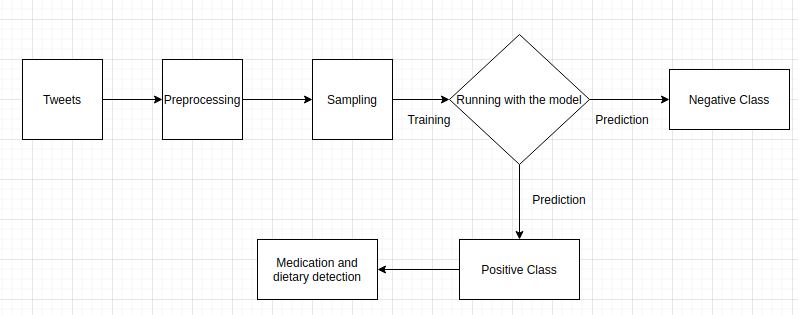
\includegraphics[width=0.99\linewidth]{Figures/system.png}
	\caption{Pipeline of the system}
	\label{fig:system-imran}
\end{figure}
